\section{Filtering and Embedding}
\label{sect:filtering-and-embedding}

In the second step we determine the overall structure that the map is going to have. To understand the requirements of this step, we need the concept of (k-)map graphs and planar graphs.

A \emph{map graph} is defined as the intersection graph of a finite number of pairwise internally disjoint regions of the plane, \ie{} its vertices are the regions and two vertices are connected by an edge if their regions touch \cite{chen2002map}. For map graphs, the number of regions that can meet in a point is unlimited, allowing for large cliques in map graphs. Although not unlimited, there are cases where more than 3 regions meet in a point in real-world maps, such as the Four Corners (Colorado, Utah, Arizona, New Mexico) in the United States.

\emph{Planar graphs} are graphs that can be drawn on the plane without its edges crossing, or, more specifically, with its edges intersecting only at their endpoints \cite{wagner2016algorithmen}. There is an equivalent definition that is remarkably similar to the one of map graphs above, namely a planar graph is a graph whose vertices are pairwise internally disjoint regions of the plane, in which two vertices are adjacent iff the respective regions share an edge, \ie{} more than just a single point \cite{chen2002map}. Obviously planar graphs are a subclass of map graphs because they have stricter requirements.

In this thesis, we want to create maps that induce planar graphs. Note that in the definition of  planar graphs we start with regions in the plane and turn them into a graph. We'll want to go in the opposite direction here: we already have a planar graph and want to turn it into pairwise internally disjoint regions whose adjacencies are equivalent to those of the vertices in the graph.

First of all, we'll need to filter the cluster graph from the previous step: complete graphs on 4 or more vertices aren't planar \cite{wagner2016algorithmen}, but we can decide on a planar subgraph of the order, \ie{} the same number of vertices, by filtering out a couple of edges. However, the graph should remain 2-connected and internally triangulated for reasons we'll outline below. Note that triangulated graphs are planar by definition.

If the graph wasn't internally triangulated, it would have holes, \ie{} internal faces on 4 or more vertices. In a corresponding map, this hole would result in lakes or rivers, which are artifacts we do not want.

\begin{figure}[H]
	\centering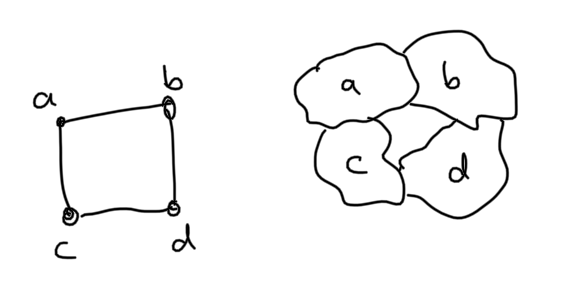
\includegraphics[height=120px]{Resources/Filtering-Hole.png}
	\caption{A 4-hole (left) and a corresponding contact representation with a lake (right) because a and d aren't allowed to touch.}
	\label{fig:filtering-holes}
\end{figure}

We also restrict ourselves to 2-connected graphs such that, in combination with the internal triangulated requirement, the outer face doesn't contain a vertex multiple times. This is due to a detail in our concrete implementation that we'll discuss later and is a restriction that could be lifted in future research.

\begin{figure}[H]
	\centering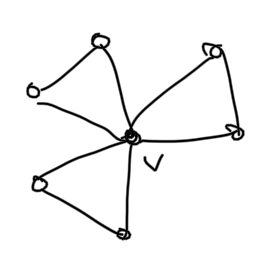
\includegraphics[height=120px]{Resources/Filtering-Connectedness.png} % TODO: Rename -> Connectivity
	\caption{A forbidden graph with a cut vertex $v$.}
	\label{fig:filtering-connectedness}
\end{figure}

Most importantly, we also decide on one of potentially many different combinatorial embeddings of the filtered graph. A \emph{combinatorial embedding} defines the cyclic orders of incident edges around the graph's vertices. \Cref{fig:filtering-embedding} shows how different combinatorial embeddings of the same graph can have vastly different appearances. Choosing a  combinatorial embedding essentially locks in the overall structure or the resulting map.
%In dynamic context: crucial to preserve mental map!

\begin{figure}[H]
	\centering
	\subfigure[clockwise]{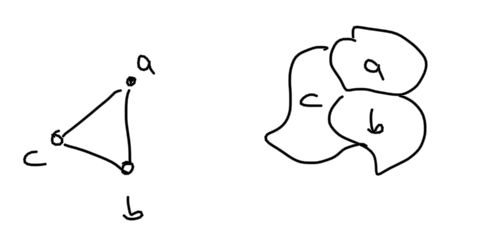
\includegraphics[width=60mm]{Resources/Filtering-Embedding-Clockwise.png}}
	\subfigure[counterclockwise]{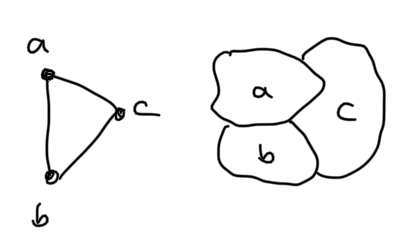
\includegraphics[width=60mm]{Resources/Filtering-Embedding-Counterclockwise.png}}
	\caption{A triangle embedded both clockwise and counterclockwise and the different resulting maps.}
	\label{fig:filtering-embedding}
\end{figure}

In summary, we take the cluster graph and filter out edges to create a vertex- and edge-weighted, 2-connected, and internally triangulated subgraph with the same number of vertices, and decide on a combinatorial embedding which we'll refer to as the \emph{filtered graph embedding}. Typically you'd want to preserve the edges with the highest weights, but other implementations are possible as well.

\begin{figure}[H]
	\centering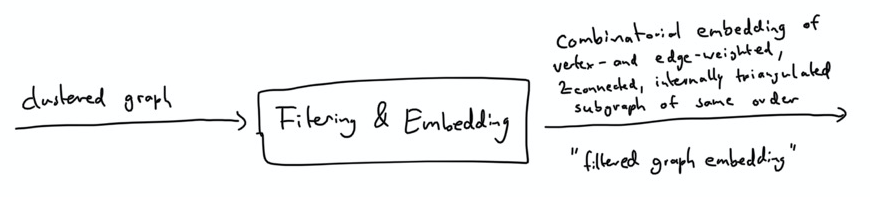
\includegraphics[width=0.9\textwidth]{Resources/Pipeline-Filtering-and-Embedding.png}
	\caption{Input and output of the filtering \& embedding phase.}
	\label{fig:pipeline-filtering-and-embedding}
\end{figure}
